 \documentclass{article}
\usepackage{fancyhdr} % Required for custom headers
\usepackage{lastpage} % Required to determine the last page for the footer
\usepackage{extramarks} % Required for headers and footers
\usepackage{graphicx} % Required to insert images
\usepackage{lipsum} % Used for inserting dummy 'Lorem ipsum' text into the template
\usepackage{amsmath,amsthm,amsxtra}
\usepackage{physymb}

% Margins
\topmargin=-0.45in
\evensidemargin=0in
\oddsidemargin=0in
\textwidth=6.5in
\textheight=9.0in
\headsep=0.25in 
\setlength{\parindent}{10ex}
\linespread{1.1} % Line spacing

% Set up the header and footer
\pagestyle{fancy}
\lhead{\hmwkAuthorName} % Top left header
\chead{\courseTitle\ : \hmwkTitle} % Top center header
\rhead{\firstxmark} % Top right header
\lfoot{\lastxmark} % Bottom left footer
\cfoot{} % Bottom center footer
\rfoot{Page\ \thepage\ of\ \pageref{LastPage}} % Bottom right footer
\renewcommand\headrulewidth{0.4pt} % Size of the header rule
\renewcommand\footrulewidth{0.4pt} % Size of the footer rule

%\setlength\parindent{0pt} % Removes all indentation from paragraphs

%----------------------------------------------------------------------------------------
%	DOCUMENT STRUCTURE COMMANDS
%	Skip this unless you know what you're doing
%----------------------------------------------------------------------------------------

% Header and footer for when a page split occurs within a problem environment
\newcommand{\enterProblemHeader}[1]{
\nobreak\extramarks{#1}{#1 continued on next page\ldots}\nobreak
\nobreak\extramarks{#1 (continued)}{#1 continued on next page\ldots}\nobreak
}

% Header and footer for when a page split occurs between problem environments
\newcommand{\exitProblemHeader}[1]{
\nobreak\extramarks{#1 (continued)}{#1 continued on next page\ldots}\nobreak
\nobreak\extramarks{#1}{}\nobreak
}

\setcounter{secnumdepth}{0} % Removes default section numbers
\newcounter{homeworkProblemCounter} % Creates a counter to keep track of the number of problems
\newcommand{\homeworkProblemName}{}
\newenvironment{homeworkProblem}[1][Problem \arabic{homeworkProblemCounter}]{ % Makes a new environment called homeworkProblem which takes 1 argument (custom name) but the default is "Problem #"
\stepcounter{homeworkProblemCounter} % Increase counter for number of problems
\renewcommand{\homeworkProblemName}{#1} % Assign \homeworkProblemName the name of the problem
\section{\homeworkProblemName} % Make a section in the document with the custom problem count
\enterProblemHeader{\homeworkProblemName} % Header and footer within the environment
}{
\exitProblemHeader{\homeworkProblemName} % Header and footer after the environment
}

\newcommand{\problemAnswer}[1]{ % Defines the problem answer command with the content as the only argument
\noindent\framebox[\columnwidth][c]{\begin{minipage}{0.98\columnwidth}\begin{center}#1\end{center}\end{minipage}} % Makes the box around the problem answer and puts the content inside
}

\newcommand{\homeworkSectionName}{}
\newenvironment{homeworkSection}[1]{ % New environment for sections within homework problems, takes 1 argument - the name of the section
\renewcommand{\homeworkSectionName}{#1} % Assign \homeworkSectionName to the name of the section from the environment argument
\subsection{\homeworkSectionName} % Make a subsection with the custom name of the subsection
\enterProblemHeader{\homeworkProblemName} % Header and footer within the environment
}{
\enterProblemHeader{\homeworkProblemName} % Header and footer after the environment
}

%----------------------------------------------------------------------------------------
%	NAME \longmapstoAND CLASS SECTION
%----------------------------------------------------------------------------------------

\newcommand{\hmwkTitle}{Homework Questions} % Assignment title
\newcommand{\hmwkDueDate}{} % Due date
\newcommand{\courseTitle}{ECE 106 - Tutorial} % Course/class
\newcommand{\hmwkClassInstructor}{Taught by: Dr. Firas Mansour and Dr. Bajcsy} % Teacher/lecturer
\newcommand{\hmwkAuthorName}{John Rinehart} % Your name
\newcommand{\sudentNumber}{} % Your name
\newcommand{\position}{PhD student in Physics Department}

%----------------------------------------------------------------------------------------
%%-----------------------------------------------------------------------------------------

%%%%%%%%%%
\newcommand{\red}[1]{\textcolor[rgb]{1,0,0}{#1}}
\newcommand{\blu}[1]{\textcolor[rgb]{0,0,1}{#1}}
\newcommand{\bs}[1]{\boldsymbol{#1}}
%\newcommand{\V}[1]{\bm{#1}}
\newcommand{\V}[1]{\Vec{#1}}
\newcommand{\A}[1]{\Hat{#1}}
\newcommand{\W}[1]{\widehat{#1}}
\newcommand{\T}[1]{\widetilde{#1}}

%\newcommand{\pd}[2]{\dfrac{\partial #1}{\partial #2}}
\newcommand {\ppds}[2]{\dfrac{\partial^2 {#1}}{\partial {#2}^2}}
\newcommand{\ppdss}[2]{\dfrac{\partial^2}{\partial #1 \partial #2}}
\newcommand{\pdtt}[3]{\dfrac{\partial^2 {#1}}{\partial {#2} \partial {#3}}}

\newcommand{\fpd}[2]{\frac{\partial #1}{\partial #2}}
\newcommand{\fpds}[1]{\frac{\partial}{\partial #1}}

\newcommand{\ignore}[1]{}

\newcommand{\der}[2]{\frac{d{#1}}{d{#2}}}
\newcommand{\vt}[1]{\Vec{\mathcal{#1}}}
\newcommand{\VP}[1]{\Vec{\mathbf{#1}}}
\newcommand{\vp}[1]{\mathbf{#1}}
\newcommand{\phas}[1]{\angle{#1}^{\circ}}
\newcommand{\er}{\epsilon_{r}}
\newcommand{\mr}{\mu_{r}}
\newcommand{\Lrw}{\Longrightarrow}
\newcommand{\refeq}[1]{(\ref{#1})}
%\newcommand{\abs}[1]{\left| #1\right|}
\newcommand{\ket}[1]{|#1\rangle}
\newcommand{\bra}[1]{\langle #1| }
\newcommand{\intas}{\int\limits_{all\;space}}
\newcommand{\intsradial}[3]{\int\limits_{#1}^{#2} #3 r^2 \mathrm{d} r}
\newcommand{\intspolar}[3]{\int\limits_{#1}^{#2} #3 sin(\theta) \mathrm{d} \theta}
\newcommand{\intsazim}[3]{\int\limits_{#1}^{#2} #3 \mathrm{d} \phi}
\newcommand{\intcz}[3]{\int\limits_{#1}^{#2} #3 \mathrm{d} z}
\newcommand{\intcx}[3]{\int\limits_{#1}^{#2} #3 \mathrm{d} x}
\newcommand{\intcy}[3]{\int\limits_{#1}^{#2} #3 \mathrm{d} y}
\newcommand{\intavcart}[1]{\int \limits_{all\; space} #1 \, \mathrm{d} x \mathrm{d} y \mathrm{d} z}
\newcommand{\bracket}[2]{\langle#1|#2\rangle }
\newcommand*{\myalign}[2]{\multicolumn{1}{#1}{#2}}

\newcommand\addtag{\refstepcounter{equation}\tag{\theequation}}
\newcommand*\diff{\mathop{}\!\mathrm{d}}


% New definition of square root:
% it renames \sqrt as \oldsqrt
\let\oldsqrt\sqrt
% it defines the new \sqrt in terms of the old one
\def\sqrt{\mathpalette\DHLhksqrt}
\def\DHLhksqrt#1#2{%
\setbox0=\hbox{$#1\oldsqrt{#2\,}$}\dimen0=\ht0
\advance\dimen0-0.2\ht0
\setbox2=\hbox{\vrule height\ht0 depth -\dimen0}%
{\box0\lower0.4pt\box2}}

%%%---
\newcommand\ointint{\begingroup
\displaystyle \unitlength 1pt
\int\mkern-7.2mu
\begin{picture}(0,3)
\put(0,3){\oval(10,8)}
\end{picture}
\mkern-7mu\int\endgroup}
%%%----
\providecommand{\abs}[1]{\lvert#1\rvert}
\providecommand{\norm}[1]{\lVert#1\rVert}

%%%%%%%%%%%%%%%

%---Packeges------------------------------------------------------------------
 %------------------------------------------------------
\usepackage{pdfsync}
\usepackage[T1]{fontenc}
\usepackage{lmodern}
\usepackage[english]{babel}
\usepackage[utf8,latin1]{inputenc}
\usepackage[T1]{fontenc}
\usepackage[usenames,dvipsnames]{pstricks}
\usepackage{epsfig}
\usepackage{pst-grad} % For gradients \usepackage{pst-plot} % For axes
\usepackage{pifont}
\usepackage{amsfonts}
\graphicspath{{IMG/}}
 \usepackage[absolute,overlay]{textpos}
 \usepackage{graphicx}
 \usepackage[bookmarks=false,pdffitwindow]{hyperref}
 \usepackage{tikz}
 \usepackage{xcolor}
 \usepackage{calc}
\usepackage{chngcntr}
\usepackage{microtype}

% Matlab code section obtained from StackExchange: http://tex.stackexchange.com/questions/75116/what-can-i-use-to-typeset-matlab-code-in-my-document
\usepackage{listings}
\usepackage{color} %red, green, blue, yellow, cyan, magenta, black, white
\definecolor{mygreen}{RGB}{28,172,0} % color values Red, Green, Blue
\definecolor{mylilas}{RGB}{170,55,241}

\lstset{language=Matlab,%
    %basicstyle=\color{red},
    breaklines=true,%
    morekeywords={matlab2tikz},
    keywordstyle=\color{blue},%
    morekeywords=[2]{1}, keywordstyle=[2]{\color{black}},
    identifierstyle=\color{black},%
    stringstyle=\color{mylilas},
    commentstyle=\color{mygreen},%
    showstringspaces=false,%without this there will be a symbol in the places where there is a space
    numbers=left,%
    numberstyle={\tiny \color{black}},% size of the numbers
    numbersep=9pt, % this defines how far the numbers are from the text
    emph=[1]{for,end,break},emphstyle=[1]\color{red}, %some words to emphasise
    %emph=[2]{word1,word2}, emphstyle=[2]{style},    
}

%----------------------------------------------------------------
\numberwithin{equation}{section}
\renewcommand{\theequation}{\arabic{equation}}



%%------------------------------------------------------------------------------------------
%	TITLE PAGE
%----------------------------------------------------------------------------------------

\title{
\vspace{2in}
\textmd{\textbf{\courseTitle\\ \vspace{0.5in}\hmwkTitle}}\\
\vspace{0.5in}\large{{\hmwkClassInstructor}}
\vspace{3in}
}
\author{\textbf{\hmwkAuthorName}\\ 
}

\date{May 28, 2015} % Insert date here if you want it to appear below your nam

%----------------------------------------------------------------------------------------
\begin{document}

\maketitle


\newpage
\tableofcontents
\newpage

%----Problems-------
\begin{homeworkProblem}[Problem 23.36]
	\textbf{Consider the electric dipole shown in Figure P23.36. Show that the electric field at a distant point on the +x axis is $E_x \approx 4k_e q a /k^3$.}

	Okay, the trick with this question is to understand what ``distant point'' means. What we mean is that the distance d that we are away from the origin along the positive x-axis is much much greater that 2a, the distance between the two charges. So, let's consider the ratio of the $\frac{2a}{d}$. Well, if $\frac{2a}{d}$ is small, then $\frac{a}{d}$ is even smaller. So, we can really see if our answer has anything that looks like a $\frac{a}{d}$ in it at the end. If it does then we will expand about a small $\epsilon \propto \frac{a}{d}$ using a Maclaurin series expansion (e.g. a Taylor series expansion about zero).

	First we need to find the electric field everywhere on the positive x-axis. Then, we need to see if we can expand. The electric field everywhere on the positivie x-axis is just given by the sum of the electric field contributions from the positive and negative charge:

	\begin{align}
		\label{}
		\vec{E}(x>0) &= k q \frac{\hat{x}}{(d-a)^2} + k q \frac{-\hat{x}}{(d+a)^2} \nonumber \\
		\intertext{I didn't use my standard method of writing $\vec{r}$, $\vec{r'}$ and $\vec{\pmb{\scriptr}}$ because it's a one dimensional problem so it's pretty easy to set up this equation. The denominator is the distance from the respective charge and the top encodes information about the strength of the charge and the direction of the electric field. Note that for x<0 this equation does not hold because the term that has (d+a) in the denominator would reference the positive charge. It's electric field would point in the positive $\hat{x}$ direction. Notice, also, that this function is not valid for anywhere off axis since then the electric field would have both an x and a y component.} \nonumber \\
		&= k q \hat{x} \big( \frac{1}{d^2(1-(a/d))^2} - \frac{1}{d^2(1+(a/d))^2} \big) \nonumber \\
		& = \frac{k q \hat{x}}{d^2} \big( \frac{1}{1-\epsilon^2} - \frac{1}{1+\epsilon^2} \big) \nonumber 
	\end{align}
	Now, we have exactly the kind of expression we were looking for. Let's expand $f^-(\epsilon) = \frac{1}{1-\epsilon^2}$ and $f^+(\epsilon) = \frac{1}{1+\epsilon^2}$.

	Expanding first $f^+(\epsilon)$:

	\begin{align}
		\label{}
		f^+(\epsilon = 0) &\approx f(0) + \frac{d}{d\epsilon}{f^+(\epsilon)}|_{\epsilon=0}\epsilon + \frac{d^2}{d\epsilon^2}{f^+(\epsilon)}|_{\epsilon=0} \frac{\epsilon^2}{2!} + \frac{d^3}{d\epsilon^3}{f^+(\epsilon)}|_{\epsilon=0} \frac{\epsilon^3}{3!} \cdots \nonumber \\
		\intertext{At this time I encourage you to evaluate these expressions yourself. I ask you to excuse me for saving myself some time.} \nonumber \\
		&= 1 - 2\epsilon + 3\epsilon^2 - 4\epsilon^3 + \cdots \nonumber \\
	\end{align}

	$f^-(\epsilon = 0)$ can be obtained in the exact same manner. However, since $f^-(\epsilon)$ only differs from $f^+(\epsilon)$ by a minus sign on $\epsilon$ we can easily write the expansion for $f^-(\epsilon)$.

	$f^-(\epsilon) \approx = 1 + 2\epsilon + 3\epsilon^2 + 4\epsilon^3 + \cdots $. Now, what we had in our earlier expression was $f^-(\epsilon) - f^+(\epsilon) \approx (1 + 2\epsilon + 3\epsilon^2 + 4\epsilon^3) - (1-2\epsilon + 3\epsilon^2 - 4\epsilon^3) = 4\epsilon +8\epsilon^3 + \cdots$. 

	Now, if $\epsilon$ is sufficiently small then $8\epsilon^3$ looks much smaller than $4\epsilon$. So much so that this smaller term is not worth considering. Thus, to first order in $\epsilon$ (that is, to the first power in $\epsilon$) our electric field at distant points is:

	$\vec{E}(x>0) = \frac{k q \hat{x}}{d^2} 4 \epsilon$. But, what is $\epsilon$? It's nothing more than $\frac{a}{d}$. Substituting this, now: $\vec{E}(x>0) = \frac{k q a\hat{x} }{d^3}$.

	This isn't quite the form in the problem statement. Now, I have to realize that $d$ is what they are calling $x$. It's the distance I have traveled along the positive x-axis. So, finally, $\vec{E}(x>0) \approx \frac{k q a \hat{x} }{d^3} $. 

	There may be a couple typos in here, but this is the idea.
	
\end{homeworkProblem}

\setcounter{equation}{0}
\begin{homeworkProblem}[Problem 23.42]

\textbf{A uniform rod of length L and total charge Q lies along the x axis as shown in Figure P23.42. (a) Find the components of the electric field at the point P on the y axis a distance d from the origin. (b) What are the approximate values of the field components when $d >>L$? Explain why you would expect these results.}

Okay, I have a little bit of time so I will try to answer this question in gory detail.

First, I am going to reintroduce the notation I've been emphasizing in this course, so far. For that purpose I am including Figure \ref{fig:vecs.eps} which I included in the document I sent to my ECE 106 tutorial students after Quiz 1. That figure makes it clear how the quantities in which we are interested related. The vector that's of primary importance is $\vec{\scriptr}$ which points from the charge generating the field to the point at which the field is to be evaluated. The two other vectors, $\vec{r}$ and $\vec{r'}$ are used to describe the positions of the point at which we want to calculate the field and the position of the charge, respectively.

Now, we have three vectors and two positions; so, these quantities are not independent. Indeed, $\vec{r'}+\vec{\scriptr} = \vec{r}$. Equivalently, \[\vec{r}-\vec{r'} = \vec{\scriptr} \addtag \]. Okay, now why are these quantities important? Well, they become important when we consider the expression of the electric field due to a point charge: $\vec{E}(\vec{r}) = \frac{k q  \hat{\scriptr}}{|\vec{\scriptr}|^2} = \frac{k q  \vec{\scriptr}}{|\vec{\scriptr}|^3}$ (note that the $\hat{\scriptr}$ changed to a $\vec{\scriptr}$ in the last expression. With a distributed charge problem, it is necessary to integrate over the charge distribution in order to determine the electric fied everywhere in space. This is analogous to how you must sum over the contributions from all discrete charges to find the electric field everywhere in space due to point charges. When we do these integrals, it is very important to keep track of the positions of the charges you are integrating over and the positions at which you want to evaluate the electric field. Note that if we are integrating over a collection of charges which form a charge distribution, we must, by extension, integrate over all the positions at which those charges can exist. This means that we must integrate over $\vec{r'}$ which is responsible for indicating where charge exists. Thus, the problem of finding the electric field due to a line of charge looks like this:

\[ \vec{E}(\vec{r}) = \int_{\text{line of charge}} \frac{k (\vec{r}-\vec{r'}) \diff q'}{|\vec{r}-\vec{r'}|^3} \addtag \]

You should recognize this as the same expression I gave earlier as the electric field due to a point charge. I have just used equation 1 to express $\scriptr$ in terms of $r$ and $r'$. I have also expressed that I will be integrating over the charge. Because that's really what's happening. I'm calculating a portion of the electric field which is due to each infinitesimal chunk of charge that's producing the total field. The positions ($r'$) over which I'm integrating will be determined by the bounds I set up in my integral. So, the integral will define where charge is. $\vec{r}$ is never evaluated until the electric field $\vec{E}(r)$ is evaluated at the point of interest. Thus, this integral over the charge, will involve integrals over $r'$ and, so, $\diff q$ should be expressible in terms of $\vec{r'}$, the coordinate that describes where the charge is located.

How can we determine what $\diff q$ is as a function of $r'$? We need to consider the geometry of the charge distribution. In this case, the charge is distributed along a line. Thus, $\diff q$ can be written as $ \diff q = \lambda \diff l$, where $\lambda$ is the linear charge density. Actually, what's really going on is that $\lambda = \frac{\diff q}{\diff l}$; the charge distribution is found by taking the ratio of the amount of charge in a little chunk of length. If the charge distribution along the line is nonuniform then the amount of charge in a little chunk of length will not be constant - i.e. $\lambda$ will not be a constant. However, in this problem, we are fortunate enough to know that $\lambda$ is a constant as a a function of length.

Now, how does $\diff l$ tie into $r'$ and $r$? Well, $\diff l$ is describing an infinitesimal motion along the path that the charge defines. Our charge distribution, in this problem, is a straight line along the x-axis. Thus, $\diff l = \diff x$. However, because I want to remember that $\diff x$ relates to the position of charges I will label it as $\diff x'$. What are the bounds of my integral? Well, $x'$, the position of my charges, are between 0 and L. Thus, my integration goes from 0 to L. So, my integral is in terms of $x'$. At this point my integral looks like: 

\[ \vec{E}(\vec{r}) = \int_0^L \frac{k (\vec{r}-x'\hat{x}) \lambda \diff x'}{|\vec{r}-x'\hat{x}|^3} \addtag \]

 What is $r'$ in terms of $x'$? Well, $r'$ describes the position of my charges. Thus, while $\vec{r'}$ can in general be expressed as  $ \vec{r'} = x' \hat{x} + y'\hat{y} + z'\hat{z}$, this problem has no charge along the $y$ or $z$ axes so the last two terms can be ignored. Our integral is a function of $\vec{r} = x \hat{x} + y\hat{y} + z\hat{z}$. We can leave it this way. That's fine. Eventually, the problem only wants to know the electric field along the y axis so we can reduce the $\vec{r}$ of interest to $\vec{r} = x\hat{x}$, but that is not necessary. If we wanted to know our electric field along the x or z axes, we could do that, too, at the end. The last thing that we should really do is find a simpler algebraic expression for the denominator of our integrand $|\vec{r}-x'\hat{x}|$. After that, we'll be in a position to solve this integral. 

\begin{align}
    \vec{r} - x'\hat{x} &= x\hat{x} + y\hat{y} + z\hat{z} - x'\hat{x} \nonumber \\
		&= (x - x')\hat{x} + y\hat{y} + z\hat{z} \nonumber \\
		\intertext{What we're interested in is $|\vec{r} - x'\hat{x}|$. But, the magnitude of a vector $\vec{a} = x_a \hat{x} + y_a \hat{y} + z_a \hat{z}$ is $|\vec{a}| = \sqrt{x^2_a + y^2_a + z^2_a}$. Thus:} \nonumber
		|\vec{r} - x'\hat{x}| =& \sqrt{(x-x')^2 + y^2 + z^2} \nonumber
\end{align}

\begin{figure}%
\centering
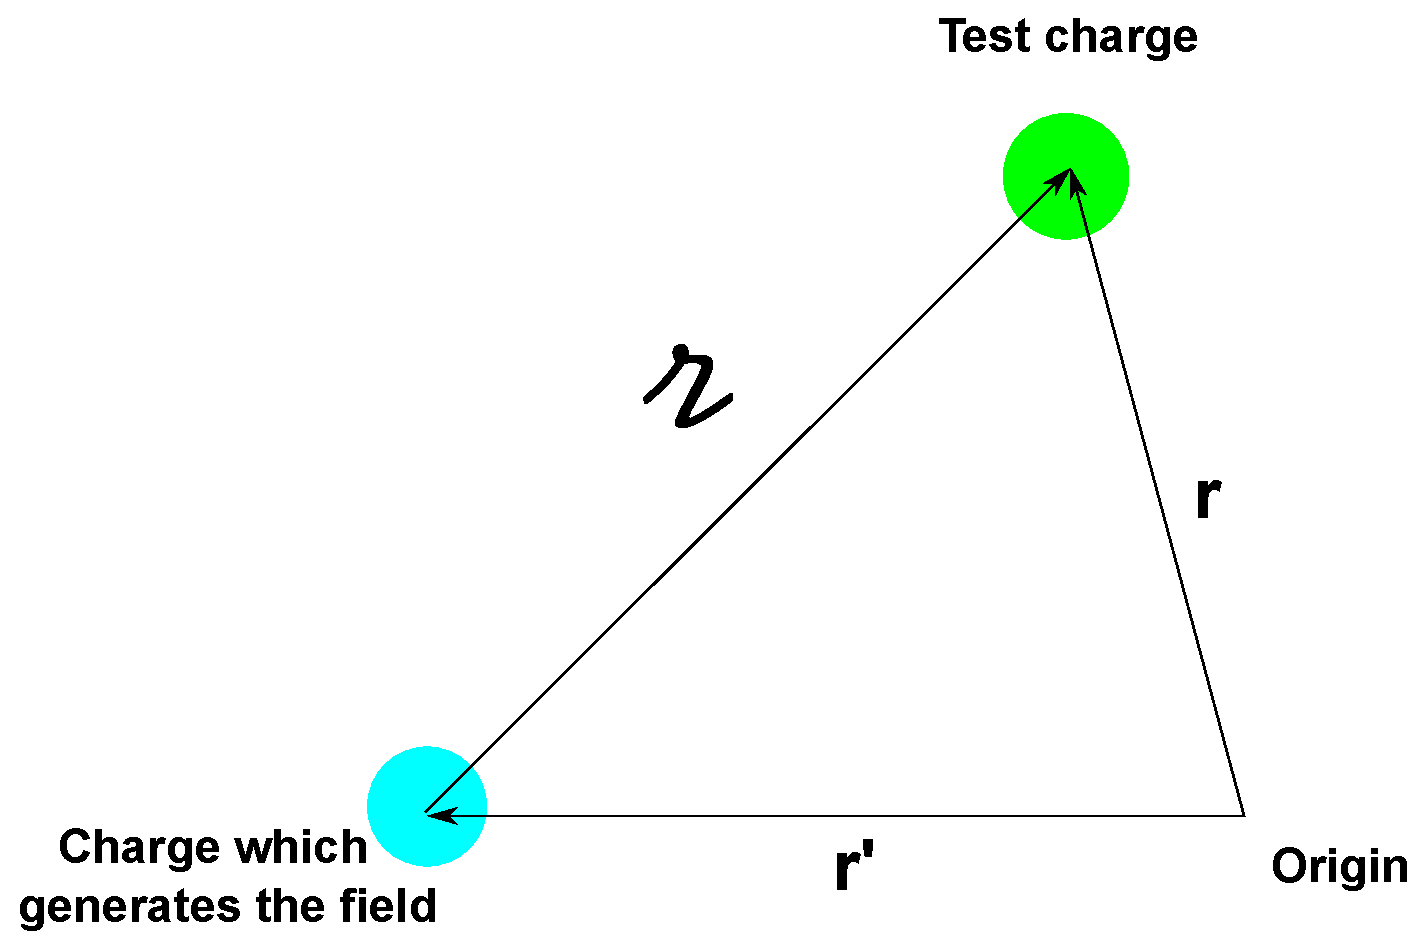
\includegraphics[width=.55\columnwidth]{vecs.eps}%
\caption{Figure used to define the vector convention for this course.}%
\label{fig:vecs.eps}%
\end{figure}

\[ \vec{E}(x,y,z) = \int_0^L \frac{k \big((x-x')\hat{x}+y\hat{y}+z\hat{z}\big) \lambda \diff x'}{\big( x'^2 + y^2\big)^\frac{3}{2}} \addtag \]

This is really three different integrals (all of which can be solved). Since I am only interested in $\vec{E}(0,y,0)$, according to the problem statement, I will set $x$ and $z$ to zero in my integral. If you don't understand why the problem statement restricts $x$ and $z$ to zero remember that we are solving for the electric field only along the y axis and that $x$, $y$ and $z$ (unprimed) are the coordinates where we are evaluating the electric field. Also, note that the solution to the integral for the y axis case looks just like that for the z axis case, which should make sense.

\[ \vec{E}(0,y,0) = \int_0^L \frac{k \big(-x'\hat{x}+y\hat{y} \big) \lambda \diff x'}{\big( x'^2 + y^2\big)^\frac{3}{2}} \addtag \]

Okay, I have everything grouped awkwardly so I'm going to pull out constants and split up the integral into two parts:

\[ \vec{E}(0,y,0) = k \lambda \bigg( \int_0^L \frac{-x'\hat{x} \diff x'}{\big( x'^2 + y^2\big)^\frac{3}{2}} + \int_0^L \frac{y\hat{y} \diff x'}{\big( x'^2 + y^2\big)^\frac{3}{2}} \bigg) \addtag \]

Technically, the $\hat{x}$ and $\hat{y}$ could come out of the integral, too, but it looks a little better, I think, to keep them in. Okay, now this looks a little complicated. However, we are only integrating over $x'$. The y is a constant with respect to the integral. Thus, the first integral looks like: 

\[ \int \frac{x \diff x}{(a^2+x^2)^{1.5}} = -\frac{1}{\sqrt{a^2+x^2}} + C \]

While the second looks like:

\[ \int \frac{\diff x}{(a^2 + x^2)^{1.5}} = \frac{x}{a^2\sqrt{a^2+x^2}} + C\].

I'm pretty sure that you can solve both of these using a u-substitution and turning the crank. I just used Wolfram Alpha. Now, we just have to plug in our bounds and we're done. Doing this yields:


\[ \vec{E}(0,y,0) = k \lambda \bigg( \hat{x} \frac{1}{y^2+x'^2}\Big|_0^L + y \hat{y} \frac{x'}{y^2\sqrt{y^2+x'^2}}\Big|_0^L \bigg) \]

Evaluating these limits:

\[ \vec{E}(0,y,0) = k \lambda \bigg( \hat{x} \big( \frac{1}{\sqrt{L^2+ y^2}} - \frac{1}{y } \big) + \hat{y} \frac{L}{y\sqrt{y^2+L^2}} \bigg) \]

This is the electric field as a function of distance along the y axis (positive and negative). Now, $\lambda$ wasn't given in the problem statement. It's not good to introduce variables for a solution, if avoidable. So, let's substitute $\lambda = \frac{Q}{L}$ since we know that $Q = \lambda L$. 

\[ \vec{E}(0,y,0) = k Q \bigg( \hat{x} \big( \frac{1}{L \sqrt{L^2+ y^2}} - \frac{1}{y L} \big) + \hat{y} \frac{1}{y\sqrt{y^2+L^2}} \bigg) \]

This is the final answer (with $d$ substituted for $y$). When $d$ (or $y$) is much much greater than L (that is: $\frac{L}{d} << 1$) what does the field look like? Well, we need to do the same trick as in the previous problem and Maclaurin expand the electric field about small $\epsilon = \frac{L}{d}$. Recognizing $\frac{L}{y}$ in our radicals in the previous expression, we write:

\[ \vec{E}(0,y,0) = k Q \bigg( \hat{x} \big( \frac{1}{L y\sqrt{(\frac{L}{y})^2+ 1}} - \frac{L}{y L^2} \big) + \hat{y} \frac{1}{y^2 \sqrt{1+(\frac{L}{y})^2}} \bigg) \]

Expressing this in terms of $\epsilon$:

\[ \vec{E}(0,y,0) = k Q \bigg( \hat{x} \big( \frac{\epsilon}{L^2 \sqrt{\epsilon^2+ 1}} - \frac{\epsilon}{L^2} \big) + \hat{y} \frac{\epsilon}{y^2 \sqrt{1+\epsilon^2}} \bigg) \]

I chose to multiply expressions by $ \frac{L}{L}$ instead of $\frac{y}{y}$ because $L$ is a fixed quantity. When I replace $\epsilon$ for $\frac{L}{y}$ want to make sure that I don't eliminate any $y$s. I am going to study the limiting case of large $y$, not small L. By multiplying by $\frac{L}{L}$ I keep the constant $L$, not the variable $y$. Now, performing a Maclaurin series expansion on the first term results in:

\[ \frac{\epsilon}{\sqrt{\epsilon^2+1}} \approx \epsilon - \frac{\epsilon^3}{2} + \cdots \]

The second term does not need to be Maclaurin series expanded. It is already in polynomial form. The last term expands like:

\[ \frac{1}{\sqrt{1+\epsilon^2}} \approx 1 - \epsilon^2/ + \cdots \]

So, finally:

\[ \vec{E}(0,y>>L,0) \approx k Q \bigg( \hat{x} \big( \frac{\epsilon}{L^2} -\frac{\epsilon^3}{2 L^2} - \frac{\epsilon}{L^2} \big) + \frac{\hat{y}}{y^2} \big( 1 - \epsilon^2/2 \big) \bigg) \]

This can be reduced to 

\[ \vec{E}(0,y,0) \approx k Q  \frac{\hat{y}}{y^2} \]

Notice that this just looks like the electric field from a point charge Q located at the origin. This is what the answer to the problem is. 

The way in which you can argue this is that for sufficiently large $y$, $\epsilon$ will be sufficiently small such that terms to higher order than $\epsilon = \frac{L}{y}$ can be ignored. I am not saying that terms of order $\epsilon^3$ don't contribute the electric field. They do. But, if I'm far enough away from the line of charge $\epsilon^3$ looks like nothing. As an example, if my charged length is 1 meter long and I am standing 100 meters away from it $\epsilon^3 = 10^ {-6}$ while $\epsilon = 10^{-2}$. The difference between $\frac{1}{100}$ and $\frac{1}{100.0001}$ is not that large. If you think that's an appreciable difference then I'll stand 1000 meters away. Then $\epsilon^3 = 10^{-9}$ and $\epsilon = 10^{-3}$. The divide between $\epsilon$ and $\epsilon^3$ grew by two orders of magnitude. I could keep doing this.

Okay. I'm done typing now. I hope that this helps.

\end{homeworkProblem}
\setcounter{equation}{0}
---------------------
%\begin{homeworkProblem}[Quiz 3, Pr. 2]
    \textbf{Charge Q is uniformly distributed over the volume of a
    hollow sphere of inner radius a and outer radius b, as shown. r is
    the distance from the center of the hollow part (the geometrical
    center of the structure).}

    \begin{homeworkSection}{2a}
        \textbf{Find the electric field inside the hollow part.}
        \\
        
        \begin{figure}[t]
            \centering
            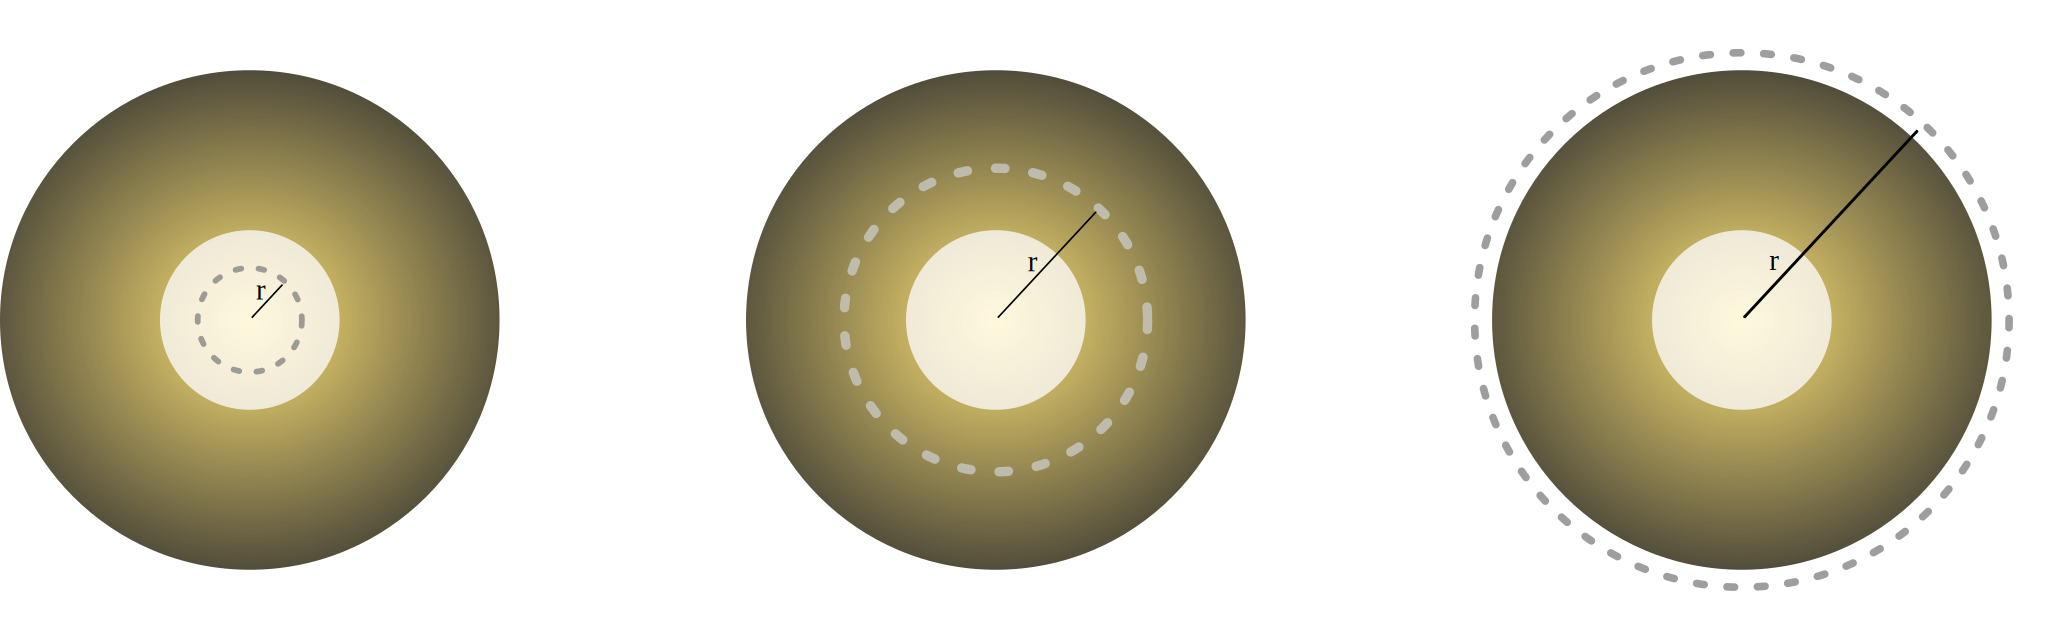
\includegraphics[width=.75\textwidth]{./img/gaussianspheres.pdf}
            \caption{Hollow, charged sphere with Gaussian spheres
            located within the hollow (left), within the charged region
            (right) and encompassing all of the charge in the sphere
            (right)}
            \label{fig:gaussianspheres.eps}
        \end{figure}

        This is a little more challenging than the previous, problems.
        Now, we are dealing with a continuous distribution of charge. In
        order to find the electric field we must use Gauss' law:
        $\oint\limits_{\text{surface}}
        \vec{E}\cdot\vec{da} = \frac{Q}{\epsilon_0}$. The way in which
        we'll use Gauss' law is we'll define a surface that takes
        advantage of the symmetry of the problem. We'll pick a surface
        whose differential area vector ($\vec{da}$) is in the same
        direction as the electric field, $\vec{E}$, for all the places
        at which we need to compute this integral. The most natural
        surface to use is a sphere.
        
        The spherical charge distribution should, through symmetry
        considerations, generate an electric field that is radially
        distributed. You can justify this by imagining rotating the
        sphere. If the sphere is perfectly symmetrical then there must
        be no way that you can tell what is ``up'' ,what is ``left'',
        etc. Thus, the electric field must be symmetric with respect to
        rotations. The only distrbution of vectors that accomplishes
        this is a radial distribution.
        
        Now, our surface, our ``Gaussian surface'', will be a sphere
        with a specified radius. In this part of the problem, we are
        only asked to compute the electric field in the region where
        $r<a$. That is, in the region where there is no electric charge.
        The way in which we'll calculate the electric field is to define
        a sphere of a certain radius ($r<a$) and we'll find out how much
        charge is enclosed inside that sphere. By relating the enclosed
        charge to the surface area of our sphere we can calculate the
        electric field. Watch:

        \begin{align}
            \label{}
            \Phi = \oint\limits_{\text{sphere}} \vec{E}\cdot\vec{da} =
            \frac{Q_{enc}}{\epsilon_0} \nonumber \\
            \oint\limits_{\text{sphere}} \vec{E}\cdot\vec{da} =
            \frac{\oint\limits_{\text{charge enclosed}}\rho dV}{\epsilon_0}
        \end{align}

        Note, that my Gaussian surface, this sphere, might enclose a
        distribution of charge. So, it's necessary for me to add up all
        the charge that might be enclosed by my sphere. That's the
        reason I have rewritten the right-hand side.

        Okay, now we can simplify the expression on the left-hand side
        of the above expression. $\vec{E}$ is, by symmetry
        considerations, directed radially outward. That is $\vec{E} =
        E(r) \hat{r}$. Now, I can also argue that by symmetry the
        magnitude of the electric field should be the same at all
        distances $r$ away from the origin. Thus, $E(r)$ is a constant
        and can be pulled out of the integral. The differential area
        element $\vec{da}$, by virtue of me having chosen a sphere as my
        Gaussian surface is $da \hat{r}$. So, it is in the same
        direction as the electric field. Thus, $\vec{E}(r) \cdot
        \vec{da} = E(r) da$, where $E(r)$ is a constant. Applying all
        these simplying results yields:

        \[
        \oint\limits_{\text{sphere}} \vec{E}\cdot\vec{da} = E(r)
        \oint\limits_{\text{sphere}} da
        \]

        The last expression is just asking for the total surface area of
        the sphere (the sum of all of the differential areas is the
        total area). Thus:
        
        \[
        E(r) \oint\limits_{\text{sphere}} da = E(r) 4\pi r^2
        \]

        Where $r<a$ is the radius of our Gaussian surface. Now, how much
        charge is enclosed by our Gaussian surface for $r<a$? Nothing!
        There is no charge for $r<a$. Thus
        $\frac{\oint\limits_{\text{charge enclosed}}\rho dV}{\epsilon_0} = $.
        Since $r \ne 0$ equation 1 (along with our simplifying
        expressions) informs us that $E(r)=0$ everywhere inside the
        hollow region (for all $r<a$). Thus, the answer to 1a is $E(r<a)
        = 0$.

    \end{homeworkSection}
    \begin{homeworkSection}{2c}
        \textbf{Solve for the electric field for outside of the sphere
        where $r>b$.}
        \\

        Okay, this part of the quiz is easier than 2b, which is why I'm
        solving it first. I will start by using equation 1, which still
        applies.
        
        \[
            \oint\limits_{\text{sphere}} \vec{E}\cdot\vec{da} =
            \frac{\oint\limits_{\text{charge enclosed}}\rho dV}{\epsilon_0}
        \]

        Okay, by the same arguments as before, I can rewrite the left
        hand side as:

        \[
            E(r)\oint\limits_{\text{sphere}} da =
            \frac{\oint\limits_{\text{charge enclosed}}\rho dV}{\epsilon_0}
        \]

        Now, though, the charge enclosed is not zero. In fact, for $r>b$
        we have enclosed all of the charge on the sphere. Can we prove
        this? Yes. Let's first consider how we would find the amount of
        enclosed charge $Q_{enc} = \oint\limits_{\text{charge enclosed
        }}\rho dV$ Well, how much charge is this? It's
        $Q = \rho * V_{\text{charged hollow sphere}}$.        What is
        the volume of the charged hollow sphere? Well, it's the volume
        of a sphere of radius $b$ minus the volume of a sphere of radius
        $a$ : $V_{\text{charged hollow sphere}} = \frac{4\pi}{3}b^3 -
        \frac{4\pi}{3}a^3$. What is $\rho$? $\rho =
        \frac{Q}{V_{\text{charged hollow sphere}}}$. It is the amount of
        charge stored per volume of the charged hollow sphere.
    
        \[
        \rho = \frac{Q}{\frac{4\pi}{3}b^3 - \frac{4\pi}{3}a^3}
        \]

        Note that this is not the same thing as:
       
        \[ \rho = \frac{Q}{\frac{4\pi}{3}(b - a)^3} \]
        
        because $(a-b)^3 \ne (a^3-b^3)$, in general. The best way to
        think about the volume (to avoid algebraic mistakes) is to
        subtract the volumes of two spheres.

        So, finally, what is the total charge enclosed by our Gaussian
        surface? Well, it's our charge density, $\rho$, times the volume
        of charge enclosed. Since our Gaussian surface is larger than
        the charged sphere, though, then $V_{\text{charged hollow
        sphere}} = \frac{4\pi}{3}b^3 - \frac{4\pi}{3}a^3$, the volume of
        the entire charged hollow sphere. And, finally, $Q_{enc} =
        \rho*V_{\text{charged hollow sphere}} = Q$, the total charge on the
        sphere.

        Okay, we already said this. It makes sense. Once our Gaussian
        surface is bigger than the charged hollow sphere then our
        Gaussian surface must enclose all of the charge. But, this mode
        of thinking will help us, later, when we try to solve 2b. Okay,
        now, $\rho$ is a constant so we can pull it out of the
        right-hand side of our expression for Gauss' law. Then, we're
        just integrating over the volume of our Gaussian surface. For a
        Gaussian surface with radius $r>b$, the Gaussian surface's
        volume is just $\frac{4\pi}{3} r^3$. Thus, our expression for
        Gauss' law can be reduced to:

        \[
            E(r) 4\pi r^2 = \frac{Q}{\epsilon_0}
        \]

        Now, $E(r) = \frac{Q}{4\pi\epsilon_0 r^2} = \frac{kQ}{r^2}$.
        This is an important result. Outside of a spherically symmetric
        charge distribution, the electric field looks like exactly that of
        a point charge located at the origin. How big is that point
        charge? Well, it's as big as the amount of charge stored in that
        spherically symmetric charge distribution. Okay, this is the
        answer for 2c. Let's tackle 2b.
        
    \end{homeworkSection}
    \begin{homeworkSection}{2b}

        Okay, we'll start with Gauss' law. I'll immediately apply the
        symmetry results to simplify the expression.

        \[
            E(r)\oint\limits_{\text{sphere}} da =
            \frac{\oint\limits_{\text{charge enclosed}}\rho dV}{\epsilon_0}
        \]

        We have the expression for $\rho$ from before.
        \[ \rho = \frac{Q}{\frac{4\pi}{3}(b^3- a^3)} \]

        Now, $\rho$ is a constant (uniform charge distribution), so I
        can pull this out of the integral. The integral on the left-hand
        side over $da$ is just the area of our Gaussian surface $\oint
        da = A = 4\pi r^2$, as usual. The most difficult thing in this
        problem is the integral over $dV$ in the right-hand side. This
        is not the volume of our Gaussian surface! We are trying to
        calculate the amount of enclosed charge. Thus, this volume
        should be the volume of the enclosed charge. At a distance $r$
        from the center, the amount of charge I have enclosed is

        \[
        V_{\text{charge enclosed}} = \frac{4\pi}{3}r^3 -
        \frac{4\pi}{3}a^3
        \]

        It's exactly the volume of my Gaussian surface \textbf{minus the
        volume of my Gaussian surface in which there is no charge}. This
        is the center of the hollow sphere. Substituting this yields:

        \[
        E(r)4\pi r^2  = \frac{1}{\epsilon_0} \bigg(
        \frac{Q}{\frac{4\pi}{3}b^3 - \frac{4\pi}{3}a^3}\bigg) \bigg( \frac{4\pi}{3}
        r^3 -\frac{4\pi}{3}a^3 \bigg)
        \]

        After a little algebra this can be rewritten as:

        \[
        E(r) = \frac{Q}{4\pi \epsilon_0 r^2} \frac{r^3-a^3}{b^3-a^3}
        \]

        This is the answer for problem 2b.
    \end{homeworkSection}
    \begin{homeworkSection}{2d}
        \textbf{Solve for the electric field at the outer surface where
        $r=b$.}
        \\

        Now, this problem is very simple. We just have to plug in $r=b$
        into our expressions for $E(r)$ from either part b or or part c.
        How come we can use either expression? Well, the electric field
        outside the sphere, for all $r>b$, is given by the answer in 2c.
        The electric field inside the sphere, for $a<r<b$, is given in
        2b. So, taking the limit as $r\rightarrow b$ both expressions
        should yield the same thing, if a limit exists. And, this is a
        fairly simple situation, that could be constructed fairly
        easily, so we hope a limit exists. It's easiest to plug $r=b$
        into the answer we got in 2c, but we could just as well plug it
        into 2b. If we do this, we obtain:

        \[
        E(b) = \frac{kQ}{b^2}
        \]
    \end{homeworkSection}
\end{homeworkProblem}

%\setcounter{equation}{0}
%--------------------- 
%\input{Problem3}
%\setcounter{equation}{0}
%----------------------
%%% ... %%%
%$\input{Problem4}
%\setcounter{equation}{0}

%\input{Problem5}
%\setcounter{equation}{0}
%\newpage
%\input{Appendix}
%%%\newpage
%%%\input{Mybib}


%----------------------------------------
\end{document}
